\chapter{Method Implementation And Results}

In this chapter the tools used, the software infrastructure and method implementation and the results collected during the analysis are reviewed.

A DDPG Agent\footnote{An agent whose actions are taken by a neural network trained with the reinforcement learning algorithm DDPG} was trained to drive in an urban environment. Checkpoints of the network's state during the training were recorded for the purpose of comparison. These checkpoints of the network were then tested with and without a simple safety-monitor in order to provide a new point of view to study AV's behaviours.

\section{Tools and software}

\subsection{Carla Simulator}

In order to have a realistic environment, with accurate physics simulation and data sensors, the open-source simulator CARLA\cite{carla}, developed by researchers at the University of Barcelona, was used. This simulator was developed with the purpose of offering an environment where AI agents can be trained to drive, with high control of the simulation parameters and the simulation of realistic sensor, which can be tuned to increase or decrease data quality, or to inject faults.\newline
CARLA is developed with a client-server architecture in mind. The \textsl{server} is basically a game, developed with \textsl{Unreal Engine 4} in C++. C++ performances are with no doubt essential to the functionality of the server: not only the environment must be simulated (including movements of pedestrians/vehicles, weather simulation\dots), but also all the data needed from the sensors attached to the system.\newline


\begin{figure}[h!]
	
\includegraphics[width=\textwidth]{img/carla.jpg}
	\caption{CARLA logo at carla.org}
\end{figure}

CARLA is currently at version 0.9.7 and huge improvements are done at every release, gaining more attention from the experts for its realism. Unfortunately, when this study started, CARLA 0.9 was recently released and the tools needed for our work couldn't be found online. Thanks to the quantity of work done for the last \textit{stable} version of CARLA, 0.8.4 was used at first.\newline
Versions prior to 0.9 have some limitations on the control one has of the simulations parameters and on the data collectable from it. This doesn't impede our study, but of course limited in some way the informations on the environment and system. Some of these problems are still present in later versions of the simulator, but most of them were solved in the transition from 0.8 to 0.9.\newline\newline
One of the main problems found was with the coordinate systems. Before version 0.9, developers were using UE4's default coordinates system which is left-handed, while the standard is considered to be right-handed. This looks like not a big deal since things could be easily solved by applying a transformation matrix. However, due to performance issues (a Python client should do the real-time processing of \textsl{loads} of data at each timestep, resulting in considerable slowdowns as a result of all the processes running at the same time), it was decided to stick with the developers' decision and convert the data during analysis phase.

Unfortunately, this version of CARLA has only 4 sensors available, which were all used during the experiments. They can be easily accessed via the Python APIs provided:

\begin{itemize}
	\item Cameras
	\begin{itemize}
		\item The \textsl{scene final} camera provides a view of the scene (just like a regular camera)
		\item The \textsl{depth map} camera assigns RGB values to objects to perceive \textsl{depth} of the environment
		\item A \textsl{semantic segmentation} is used to classify different objects in the view by displaying them in different colors, according to the object's class
	\end{itemize}
	\item Ray-cast based Lidar
	\begin{itemize}
		\item Light Detection and Ranging is use to sense the environment and measures distance from objects by illunating the target with laser beams and measuring the time reflected light needs to "go back" to the sensor
	\end{itemize}
\end{itemize}

The three cameras were used during the training phase of the network. Three \textsl{scene final} cameras are attached to the car to actually \textsl{see} the environment (one on the front and one per side). The \textsl{depth map} camera allows the car to get a colormap of the distances from objects in the scenario.
The \textsl{semantic segmentation} provides image classification features by querying the server for ground-truth values. This is with no doubt a semplification of a real system, where the most powerful image-classification softwares are essentially other neural networks trained separately. At the same time a misclassification can be considered as an error of the control system: if the safety monitor detects the possible hazard it will not "correct" the misclassification but it must react fast and safely to avoid the possible consequences of it, therefore this simplification won't have an impact on the overall method.\newline

A ray-cast based Lidar is the only other sensor available for this version of CARLA. Parameters of this sensor can be easily tuned to simulate real lidars such as the \textsl{Velodyne LiDAR} or to simulate faults such as low data quality, noisy data or data loss\dots This data are generated using the \textsl{Point Cloud}\cite{pointcloud} format

In the simulations, due to the high hardware resources requirements to simulate a real LiDAR, a slightly modified version of the \textsl{Velodyne64 LiDAR} is implemented with the following parameters:

\begin{itemize}
	\item Channels = 64
	\begin{itemize}
		\item The number of laser beams used by the system. These lasers are distributed over the vertical axis. The more the lasers are, the more accurate will be the scannings
	\end{itemize}
	\item Range = 75m
	\begin{itemize}
		\item Lasers' range in meters
	\end{itemize}
	\item Rotation Frequency = 15 Hz
	\begin{itemize}
		\item This parameters define the rotation frequency (in Hz) of the scanning beams.
	\end{itemize}
	\item Points Per Second = 1.000.000
	\begin{itemize}
		\item The actual number of points generated each frame by the sensor
	\end{itemize}
	\item Vertical FOV bounds (height = 24m, low = -2m. Distances are relative to the position of the sensor)
	\begin{itemize}
		\item Maximum and minimum height of the scannings
	\end{itemize}
\end{itemize}

The simulator provides Python APIs not only to modify sensors, but also to have a great control on what is being simulated, such as seeds definition for the spawning points and the behaviours of pedestrians and vehicles, and on the state of \textsl{"actors"} in the scene such as their position, their speed\dots. All these data are directly provided by the simulator with ground-truth values. These kind of measurements can be simulation-related, such as the simulation time-step, or the FPS. Actors-related measurements include for example vehicles' speed, intensity of collisions (if any) and the 3D acceleration vector.\newline

While this tool was being tested a problem was found with the LiDAR sensor data that is still not resolved.\cite{lidarbug} 
The bug resulted in the vehicles' bounding boxes to be distorted when moving, providing very poor data.
After some research an improved version of the simulator was found, where the bounding boxes for each vehicle were redefined to provide accurate data.\cite{carlapro} As of today, developers are working on this issue but it is still unresolved without manual intervention on the source code.


\subsection{Controller Implementation}

The main component needed for the Controller implementation is the neural network that will be in charge of deciding the action to perform to drive the car. We looked for a framework with the following characteristics

\begin{itemize}
	\item[1] Training code must be available
	\item[2] No critical issues in the codebase
	\item[3] Provide an environment to interface the network with CARLA
	\item[4] Provide a default training strategy
\end{itemize}

After analyzing all the machine-learning related projects for CARLA, we chose the reinforcement-learning framework \textsl{Coach}, developed by \textsl{Intel AI Lab}.\cite{coach}

This framework satisfies all the requirements listed above: it is distributed as an \textsl{editable Python package}. The development team behind this project assure us the quality of the product. Moreover, several presets are available as a starting point. Two of these presets offer an interface to the CARLA simulator, as well as a default training strategy, which is exactly what we required.

These presets implement the \textsl{Deep Deterministic Policy Gradient} algorithm, proposed in 2015.\cite{ddpg} This algorithm proved to perform well in tasks such as car driving, as shown in the original paper, and it's specifically adapted to perform in environments with continuos action space, such as the one we are considering.

\begin{itemize}
	\item[P1)] The first preset uses a single, front camera to perceive the environment, and the other data augmentation cameras provided by CARLA. The agent resulting from using this preset will likely not have any sense of depth created by the regular camera and will rely solely on the depth camera
	\item[P2)] This preset uses all the cameras available in CARLA and have a much more interesting architecture since the car is equipped with three regular cameras (Front, Left, Right) and all the data augmentation cameras available in CARLA, listed in the previous section
\end{itemize}

The usage of the data augmentation cameras (depth and semantic segmentation) allows us to ignore objects misclassifications (e.g. labeling a pedestrian as a light pole) as well as some other easinesses such as computing distances from objects. As pointed in the previous section, this is indeed a simplification of a real architecture, where object detection modules are neural networks themselves, that must be trained in advance and tested separately. However, again, a misclassification will probably cause the Controller to behave in unexpected manners that the Safety Monitor must be able to detect and possibly correct.

Unfortunately, the first preset suffers from an issue that causes the car to stop throttling, while being positively rewarded\cite{coachIssue}. It would have been interesting to test this preset as well, to understand what's the impact on the effectiveness of the Safety Monitor with respect to the quantity of data available to the network.\newline

It's important to notice that our goal \textsl{is not} to build the \textsl{"perfect"} agent, nor the perfect autonomous cars. The codebase was studied but, due to reasons of time, we could not inspect all the details of the provided implementation. This framework was used as an example to demonstrate the concepts described in this work.


\subsection{Safety-Monitor Implementation}

In order to start the experimental activity, we needed a software capable of processing LiDAR data to map the environment and sense the obstacle. Moreover, this software needs to be \textsl{real-time} and capable of interacting with CARLA. The latter is obvious: whenever an alert is raised, the \textsl{"brake"} command must be sent to the CARLA server. The first required some reasoning: one could think to record the LiDAR data in advance and then run the simulations feeding the Monitor with these data. Unfortunately this approach can not work: this comes from the fact that we are not interested in having a 100\% prediction accuracy, but also in the \textsl{goodness} of the safety-measure adopted by the Monitor. The same measurement in two different simulations could give \textsl{slightly} different results, that could cause the Monitor to behave in a completely different way than the way it could have behaved using the \textsl{real time} data produced during the simulation. If the accuracy of measurements is strictly dependent on the simulator used for the experiments (CARLA is improving at every release on this side), we could not ignore the effects that a brake can have on a single run.

In order to develop a decent Safety-Monitor, a research on the best, \textsl{"not-neural-network"} techniques was conducted, as well as a research on the open-source instruments available. The choice fell on the \textsl{Point Cloud Library}\cite{pcl}, an open-source library specifically dedicated to the processing of Point Cloud data, developed using C++ to achieve great performances when processing huge amount of data.
This library was first released in 2011\cite{pclwiki} and it's been improved at every release, also thanks to the big community testing and debugging the new features.

This library offers a multitude of functions that implements the most known techniques for Point Cloud processing. The steps to follow in order to develop an object-detection module are the following:

\begin{itemize}
	\item[1)] Downsampling
	\begin{itemize}
		\item[$\rightarrow$] The data generated by a single scan can contain more hundreds of thousands records, with possibly a lot of redundancy and noise. A downsample is usually necessary as a preliminary step to discard all the \textsl{"useless"} data. After some reasoning, the Voxel Grid Filter was chosen for this step
	\end{itemize}
\end{itemize}

\begin{itemize}
	\item[2)] Ground Segmentation
	\begin{itemize}
		\item[$\rightarrow$] After the downsampling (if needed), the first mandatory step is to filter the data that are useless for the purpose of object detection, such as points relative to the ground. These point must be filtered in order to separate the ground from the objects we want to detect.
		In our implementation this is done using the RANSAC\footnote{Random Sample Consensus} algorithm\cite{ransac}, a technique to separate \textsl{"inliers"} (i.e. data whose distribution is characterized by the model's parameters) from \textsl{"outliers"} (i.e. data that don't have a representation in the chosen model)
	\end{itemize}
\end{itemize}

\begin{itemize}
	\item[3)] Clustering
	\begin{itemize}
		\item[$\rightarrow$] This final step is required to effectively identify what is an object in the scene, and what data points are relative to the same object. This can be done using clustering algorithms based on the distance among points. We chose the Euclidean Clustering Algorithm, a range search algorithm based on the euclidean distance between points, with the assumption that \textsl{very dense} points represent the same object
	\end{itemize}
\end{itemize}

\begin{itemize}
	\item[4)] Object Tracking and Avoidance
	\begin{itemize}
		\item[$\rightarrow$] Objects detected in the first three steps must be tracked over time in order to recognize if two objects observed in two consecutive steps, are actually the \textsl{same} object, usually using physical models to predict their behaviour over time, such as the Kalman Filter, and combine this model with a failure-prevention routine
	\end{itemize}
\end{itemize}

Unfortunately, implementing a Kalman Filter for such a complex model would have been too much time-consuming, alting our study. Therefore we simplified the object-detection and the failure-prevention routine in this way:

\begin{itemize}
	\item Only data \textsl{in front of} the car are recorded. This is a huge semplification of the model, as the Monitor now can only detect obstacles ahead of the car. However, this will for sure have an impact on the effectiveness of the Safety Monitor, but the concepts explained in the previous section still holds
	\item The failure-prevention routine implemented takes inspiration from the Responsibility-Sensitive Safety model proposed by Mobileye, an Intel company.\cite{rss}
	If an object is detected, its speed relative to the system is computed. If the distance travelled by the system in 1 second  plus the braking distance is greater than the distance travelled by the object plus the distance between the system and the object, a safety brake is applied.
\end{itemize}

Since the Safety-Monitor is developed in C++, both for taking advantage of the Point Cloud Library and due to performance reasons, an infrastructure to exchange data with CARLA was developed.

The software is composed of a C++ server that receives LiDAR Point Clouds from the CARLA client. This data are processed as in the steps above (with the semplification described) and, if needed, an alert is sent back to the client. If the message received by the Monitor is an alert, the actions of the Controller are ignored and a brake is performed.

The object detection module is inspired by an open-source project developed by Engin Bozkurt\cite{LOD}. The codebase was deeply modified to adapt the detection algorithm parameters to fit our needs and to interact with CARLA.

We are conscious that this Monitor will likely not achieve "state of art" performances and it's likely to produce a lot of \textsl{false positives}. This aspect may have some consequences on the traning efficacy, but the concepts explained in this work still holds.

\section{Experimental Activity}

In this section is described how the methodology developed in the previous chapter was implemented, and the technical problems found during the implementation.

The Controller was trained in an urban environment, with the default strategy provided by \textsl{Coach} in order to generate four checkpoints to be subsequently tested.

Scenarios were generated using the 152 spawn points\footnote{Coordinates in the map in which the car will start its ride.} provided by Carla.
For each spawn point, a default setting and three variations of it were generated:

\begin{itemize}
	\item[h0)] \textsl{Default Setting}: the map is generated using the \textsl{same} conditions in which the Controller was trained, with 30 pedestrians and 15 cars
	\item[h1)] \textsl{Pedestrians Setting}: the map is generated increasing the number of pedestrians from 30 to 60
	\item[h2)] \textsl{Vehicles Setting}: the map is generated increasing the number of vehicles in the environment from 15 to 30
	\item[h3]) \textsl{Pedestrians and Vehicles Setting}: the map is generated merging $h1$ and $h2$, resulting in an environment with 60 pedestrians and 30 vehicles
\end{itemize}
	
For repeatibility, and consistency across the variations, 152 couples of unique seeds\footnote{These seeds are used in the generation of pedestrians and vehicles} were generated, each of them was associated to a starting point. This allows to have the same seed, for the same starting point, using different variations.

In general, it may require a huge amount of time for a crash to happen. For this reason, in order to demonstrate the concepts explained in this work, it was defined a maximum running time of 15 minutes, after which the System's task is considered succeeded.

In the first phase of the analysis, four checkpoints generated were tested according to the methodology described in section 3.
Since the \textsl{Coach} project is open-source, the codebase was freely available. This allowed us to use \textsl{software probes} to monitor the Controller's activity.
The source code was modified adding some instructions to write all the needed data into different file for each run:

\begin{itemize}
	\item The starting point and seeds of the Scenario
	\item Actions taken by the Controller
	\item If there is a collision, with what
\end{itemize}

Modifying the source code may in general result in a worsening of the overall performances, and the accuracy of results. Fortunately, the CARLA simulator provides an option to run the simulations at a \textsl{fixed-time step}. This was set at its minimum: 10 FPS\footnote{Frames Per Second}, to assure that all the data received from the server are \textsl{timely} and \textsl{correct}. This also serves as a mean for \textsl{repeatibility} of tests: a \textsl{variable time-step} may introduce randomness in data since we have no control over it.

The first training phase and the Controller testing required circa 1 month to be performed.\newline

The second step was to test the effectiveness of the Safety-Monitor for each checkpoint.

The source code was once again modified to create two separate, concurrent processes: one takes LiDAR data from the CARLA server and sends them to the Safety-Monitor server; the other waits for the response of the Safety-Monitor to check whether a brake is needed.

The LiDAR data are generated by the CARLA server at each frame. THe workload for data generation relies solely on the CPU, resulting in very much slower execution times. Unfortunately, CARLA suffers from a bug which causes data to be inaccurate, if FPSs are lower than 10. This required a powerful machine to guarantee the lower bound of 10 FPS.
The source code was once again modified to insert software probes in the codebase to gather informations about alarms raised by the monitor.

Runs recorded in the first step are now repeated observing the Safety-Monitor's behaviour. All the alerts raised during the run are considered \textsl{false positive}. The emergency brake is enabled 2 seconds before the collision, to estimate the amount of \textsl{true positives}.

This approach, allows us to estimate the goodness of the Safety-Monitor in its operational environment.\newline

After the first phase is concluded, data gathered are processed to compute the measures listed in the previous Chapter:

\begin{itemize}
	\item \textsl{Controller's Checkpoints}:
	\begin{itemize}
		\item[-] Mean Distance Between Failures
		\item[-] Mean Time Between Failures
		\item[-] Failure Rate
		\item[-] Reliability
	\end{itemize}
	\item \textsl{Safety-Monitor}:
	\begin{itemize}
		\item[-] True Positive Rate
		\item[-] False Negative Rate
		\item[-] False Positives per Meter
	\end{itemize}
\end{itemize}

At this point, training is resumed from the last checkpoints using the strategies described before, and the measurement process is repeated identically.

Some of the strategies defined requires the training to be done \textsl{with} the Safety-Monitor, resulting in very low execution times. This phase took 2 months, after which the training was stopped.

The numerical results collected can be compared to check if the network is learning properly and how the Safety-Monitor's effectiveness changes when the network improves.

The collected results are presented and compared in the next section.

\section{Results}

\subsection{Phase 1 - Controller Testing}

The data collected are saved in separate files for each run and processed using Python scripts, computing the measures listed in Chapter 3.

The measures collected are compared to check the goodness of the Controller and changes in the effectiveness of the Safety-Monitor over the neural network's checkpoints.

Since the Checkpoints were tested in the \textsl{same} scenarios, the distances travelled for each scenario were plotted to check if meters travelled are increasing and if there are scenarios somehow \textsl{"favorable"} or extremely \textsl{"hard"} for the system. This first step allows testers to filter between critical scenarios and easy scenarios. Ideally, given a Scenario $x$, if the distance travelled by the Controller in $x$ is lower than the average distance travelled in all the checkpoints, there may be two cases:

\begin{itemize}
	\item[1)] In the case that the Controller always travel the same distance in all the checkpoints before crashing, there may be a hazard that the Controller has not learned to handle
	\item[2)] In the case the distance travelled fluctuates in a certain (small) interval, the happening of a crash may depend from the inital conditions
\end{itemize}


Regardless of the case, with this approach it's easy to see which scenarios make the Controller crash soon, and they can be examined individually with more attention.

It is important to keep in mind that if a trend is observed when testing different Checkpoints, e.g. a scenario in which the Controller \textsl{always} performs extremely good or extremely bad, an analysis of the specific case is needed, in both of the cases.

The reason is obvious for "bad" runs, for the reason listed above. It may seem counter-intuitive, but repeated "good" runs in the same scenario requires particular attention. An analysis of the correlation between performances and initial conditions is mandatory, and it may be demonstrated or confuted with this approach. A more complex case is when the System finds a \textsl{"lucky pattern"}, for example 

\begin{minipage}[c]{\textwidth}
	\includegraphics[width=\textwidth]{simulations/gen1/standard/distance-travelled-figure.pdf}
	\captionof{figure}{Meters travelled by the Controller in the first checkpoint}

	\includegraphics[width=\textwidth]{simulations/gen4/standard/distance-travelled-figure.pdf}
	\captionof{figure}{Meters travelled by the Controller in the fourth checkpoint}

\vspace{0.5cm}
The order of magnitude is quite different between the two checkpoints and in one scenario it has been reached the maximum length defined for these experiments. These figures are just demonstrative of the improvement of the Controller over checkpoints.
\end{minipage}

The use of a \textsl{fixed time-step} when running the simulations, i.e. the simulation time elapsed between two steps of the simulation is fixed and known, gives us knowled of the interval of time between two consecutive actions: observing how many actions the Controller has taken it's possible to compute the total time of a single run.

In this way, we are able to easily approximate the \textsl{Reliability Function} for each Checkpoint.

\begin{figure}[h!]
	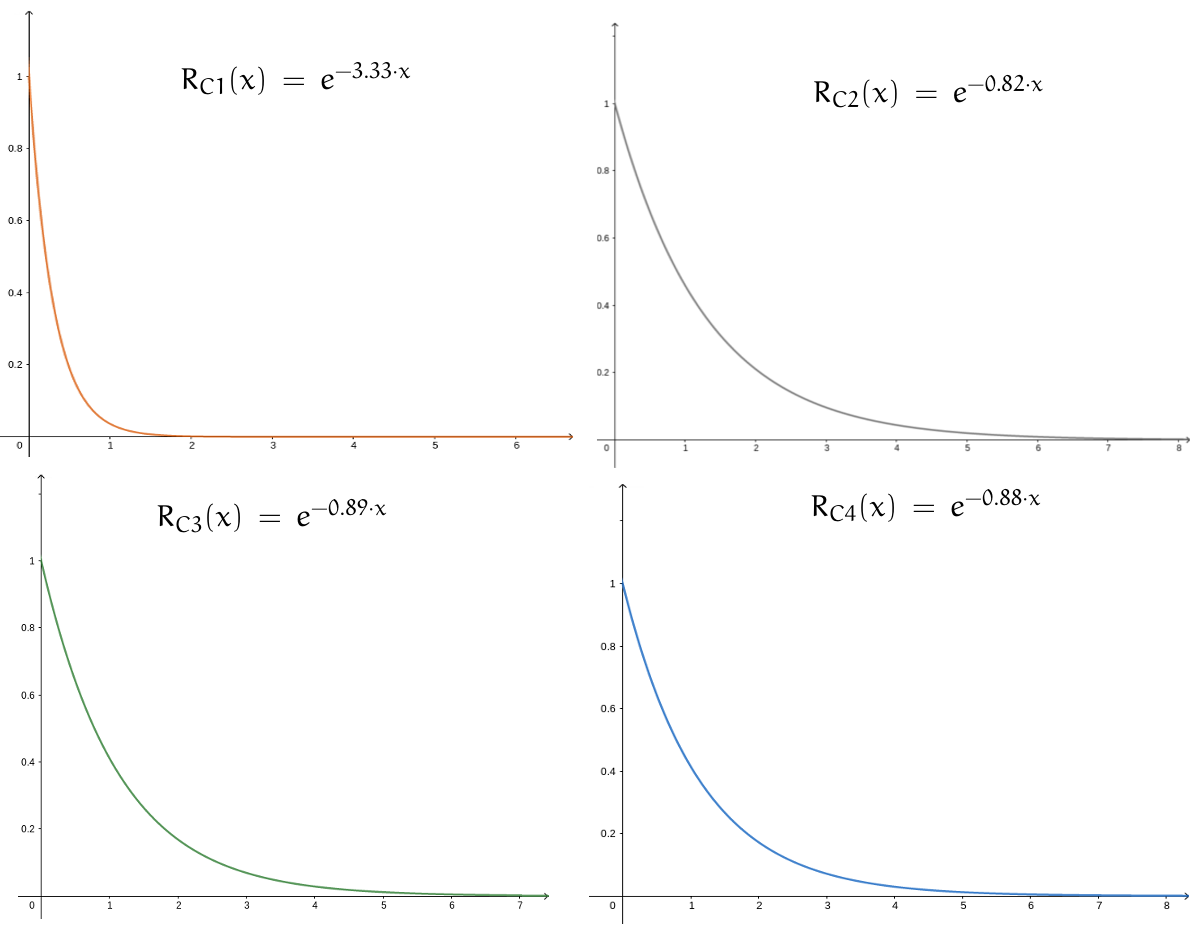
\includegraphics[width=\textwidth]{img/reliability-comparison.png}
	\caption{Graphics that shows the probability $y$ of the system being operational, after $x$ minutes of operation}
\end{figure}

As we expected, the MTTF of the first checkpoint is very low (20 seconds) and increases over Checkpoints. Surprisingly, the second Checkpoint seems to have better performances (higher MTTF) than Checkpoints 3 and 4. However, analyzing a subset of the runs in which the second Checkpoint achieved very good performances in terms of time to failure and distance travelled, it can be seen that its driving is way more dangerous than the other two, resulting in reckless runs, with sudden steer and disrespect of road rules.

Fortunately, as we will show with the results collected in phase 3, the Controller managed to overcome this problem.\newline

The same behaviour is observed for distances travelled by each Checkpoint: longer runs are actually runs in which the car travels more meters. This assure us that the system is not \textsl{"cheating"}: a longer execution time may result from the car not moving. Computing the average distance travelled by each Checkpoint in each difficulty level, allows us to approximate the Reliability Function in terms of kilometers travelled before crashing.

Moreover, the observed progresses in the \textsl{mean distance to failure} seems to follow the progresses of the \textsl{mean time to failure}, which is another assurance of the correspondence between the two metrics.

\begin{figure}[h!]
	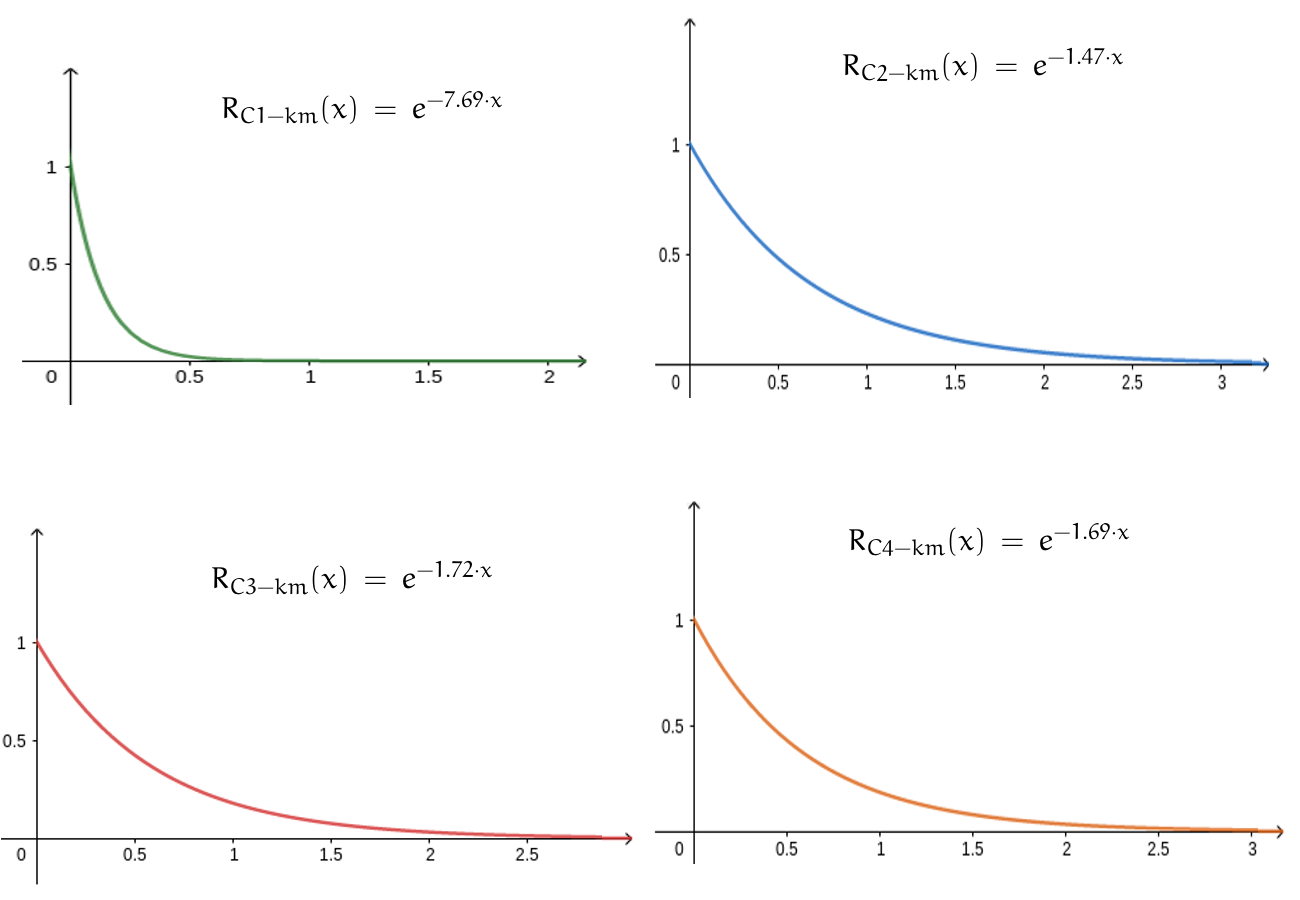
\includegraphics[width=\textwidth]{img/reliability-meters-comparison.png}
	\caption{Graphics that shows the probability $y$ of the system being operational, after $x$ kilometers}
\end{figure}

As another mean to analyze the Controller's behaviour over Checkpoints, since CARLA provides means to record the kind of object with which a collision occured, ratios of kind of object collided with respect to total collisions are computed for each Checkpoint, for each level of difficulty.
This procedure serves multiple purposes:

\begin{itemize}
	\item[1)] To monitor whether the Car crashes with obstacles, indicating that it tends to go off-road by crashing with walls, light poles, fences\dots
	\item[2)] To monitor how the Car reacts to diverse level of difficulty, e.g. if we increase the number of pedestrians and we observe for example less collisions with pedestrians, it may be an indicator that the System is capable of avoiding collisions with people.
	\item[3)] Understand the System's ability to avoid crashes with specific "objects" (pedestrians, vehicles and generic obstacles)
\end{itemize}

\begin{figure}[h!]
	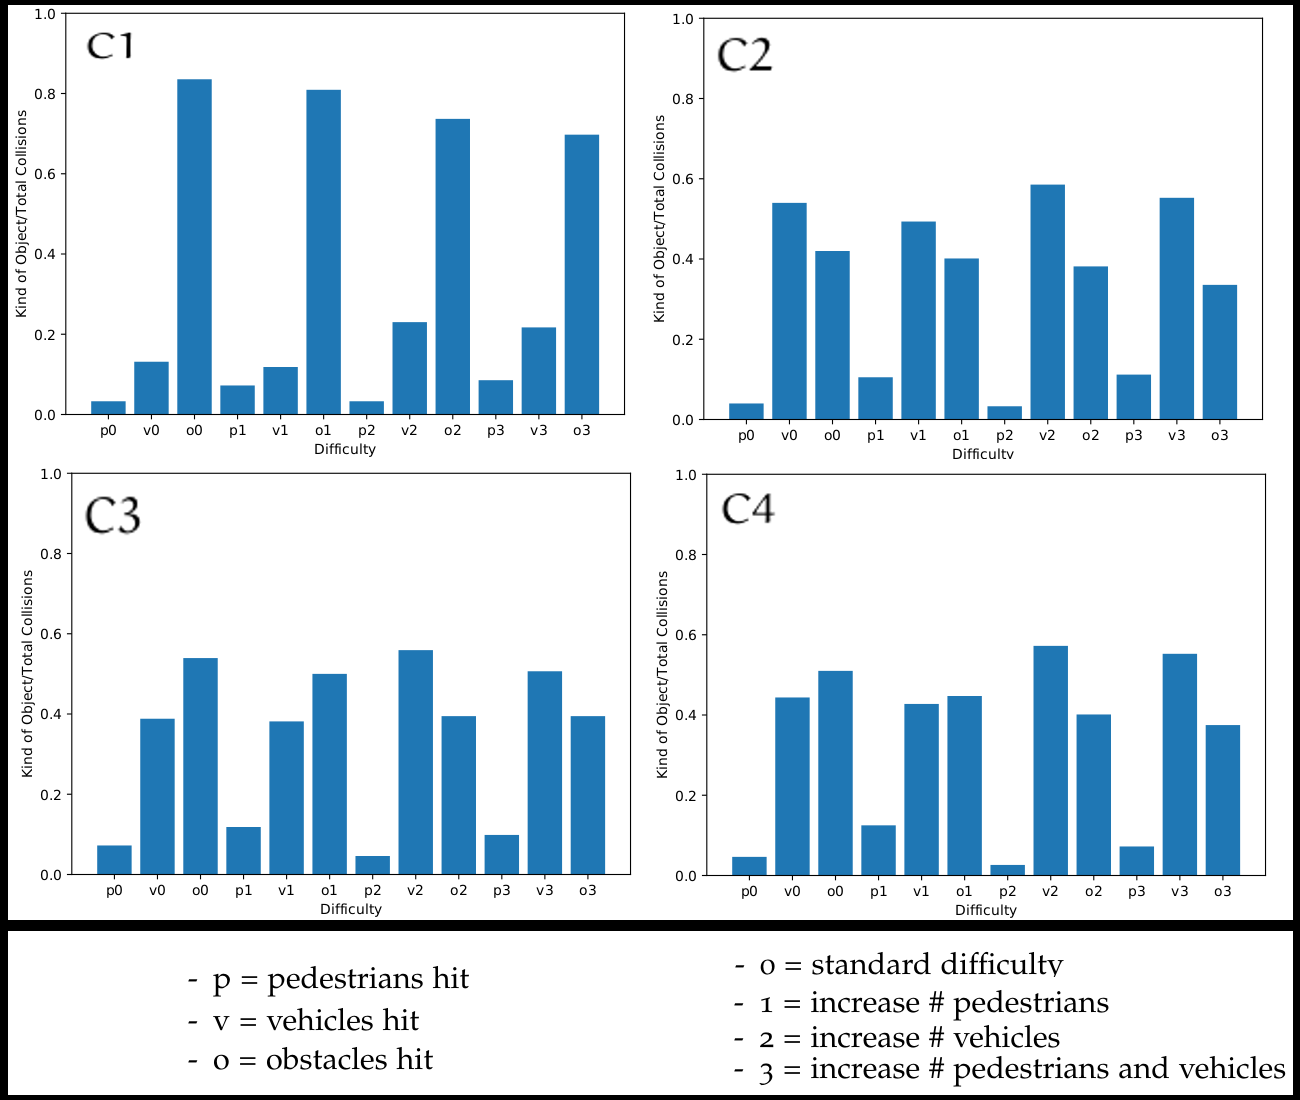
\includegraphics[width=\textwidth]{img/hit-ratios.png}
	\caption{}
\end{figure}

These diagrams are useful to have an overlook of how the System performs when changing the difficulty of the Scenario while being trained and to observe correlations between the kinds of collision and the Checkpoints.
As we could expect, the first Checkpoint mostly collides with off-road obstacles, indicating poor driving skills of the Controller.

It also seems that there is a tendency in which the ratio of collisions with generic obstacles follows the overall Checkpoint's performances.
Observing this diagram and those of the Reliability Function, it can be seen that C1 (lowest MTTF), tends to crash against obstacles, C2, which had the best performances in terms of MTTF and MDTF, has the lowest ratio of collisions against obstacles. C3 increased the ratios of these collisions, coeherently with its worsening of the MTTF/MDTF, which is subsequently lowered by C4.

Moreover, the increasing or lowering of the hit ratios with a specific kind of object, follows the features of the difficulty chosen. This means that the crashes observed are strictly dependent on the environmental conditions.

This aspect is useful for the definition of more complex difficulties. These measures also allows to detect correlations between the increase/decrease of kind of collisions.\newline

With the methodology defined for the first phase, combining the definition of the Scenarios, the difficulty levels and the metrics chosen, allows to observe many features of the Controller without actively observing its executions. Moreover, combining the few metrics chosen it is possible to have an overlook of possible correlations between environmental conditions, initial conditions, and Checkpoints.

\subsection{Phase 2 - Monitor Testing}

Dati del Monitor


\subsection{Phase 3 - Retraining and Retesting}

DATI DELLA RETE RI-ADDESTRATA. VANTAGGI DI TRAINING PIU` PUNITIVO E FALLIMENTO DEL TRAINING CON MONITOR



MIEI REMINDER:


\begin{itemize}
	\item[-] p = pedestrians hit
	\item[-] v = vehicles hit
	\item[-] o = obstacles hit
\end{itemize}

\begin{itemize}
	\item[-] 0 = standard difficulty
	\item[-] 1 = increase \# pedestrians
	\item[-] 2 = increase \# vehicles
	\item[-] 3 = increase \# pedestrians and vehicles
\end{itemize}




\begin{itemize}
	\item Generazione 1:
	\begin{itemize}
		\item MDBF: 131,67
		\item MTTF: 19,39
	\end{itemize}
	\item Generazione 2:
	\begin{itemize}
		\item MDBF: 579,37
		\item MTTF: 67,07
	\end{itemize}
	\item Generazione 3:
	\begin{itemize}
		\item MDBF: 594,94
		\item MTTF: 67,72
	\end{itemize}
	\item Generazione 4:
	\begin{itemize}
		\item MDBF: 677,98
		\item MTTF: 72,71
	\end{itemize}
	\item Generazione Pro:
	\begin{itemize}
		\item MDBF: 1108,86
		\item MTTF: 124,6
	\end{itemize}
	\item Generazione NonPro:
	\begin{itemize}
		\item MDBF: 994,31
		\item MTTF: 111,42
	\end{itemize}
	
	\vspace{1cm}
	
	
	$R_{C1}(x)\: =\: e^{-3.33\cdot x}$\newline\newline
	$R_{C2}(x)\: =\: e^{-0.82\cdot x}$\newline\newline
	$R_{C3}(x)\: =\: e^{-0.89\cdot x}$\newline\newline
	$R_{C4}(x)\: =\: e^{-0.77\cdot x}$
	
	
	
	$R_{C1-km}(x)\: =\: e^{-7.69\cdot x}$\newline\newline
	$R_{C2-km}(x)\: =\: e^{-1.72\cdot x}$\newline\newline
	$R_{C3-km}(x)\: =\: e^{-1.69\cdot x}$\newline\newline
	$R_{C4-km}(x)\: =\: e^{-1.47\cdot x}$
	
	
	
	
\end{itemize}


